% appendix.tex
% Supplementary material: empirical validations of assumptions used in
% the main-text derivations, plus material that is too dense for the
% main body but useful for replication.

\section{Empirical cross-term diagnostic}
\label{sec:supp-cov}

The variance correction of Eq.~\eqref{eq:scale} rests on the
assumption $\Cov[\teps_i, g_m] \approx 0$, which is what allows the
derivation to drop the cross-term in the expansion of $\Var[g_i]$. Because the per-asset JumpHMM marginals are
fit to each asset's full growth-rate history, including its
market-correlated component, the assumption is not automatic: a
generator that picked up a residual market loading would invalidate
the closed-form scaling. We tested the assumption empirically by sampling $R = 100$
innovation paths $\teps_i^{(r)}$ per ticker from each generator and
computing the normalized cross-covariance against the real SPY path:
\begin{equation}
  \mathrm{cov}^{\mathrm{norm}}_i
  = \frac{1}{R} \sum_{r=1}^{R}
    \frac{\Cov[\teps_i^{(r)},\, g_m]}{\sigma_{\teps,i}\, \sigma_m}.
\end{equation}
Per-ticker values were plotted as histograms in
Fig.~\ref{fig:cov_diag}. Across the $423$ tickers, the full-return
JumpHMM generator (used by the hybrid and naive composers) sat
within $\pm 0.006$ of zero with a per-ticker mean bias of
$1.5\times 10^{-4}$ (Fig.~\ref{fig:cov_diag}); the residual-fit
JumpHMM generator (used by the JumpHMM-on-residuals composer) and
the Gaussian baseline were also centered at zero (mean $7\times 10^{-5}$ and $2.3\times 10^{-4}$
respectively, Fig.~\ref{fig:cov_diag}). The
independence assumption was therefore satisfied to within sampling
tolerance for all three generators, and the derivation of
Eq.~\eqref{eq:scale} held in practice.

\begin{figure}[t]
  \centering
  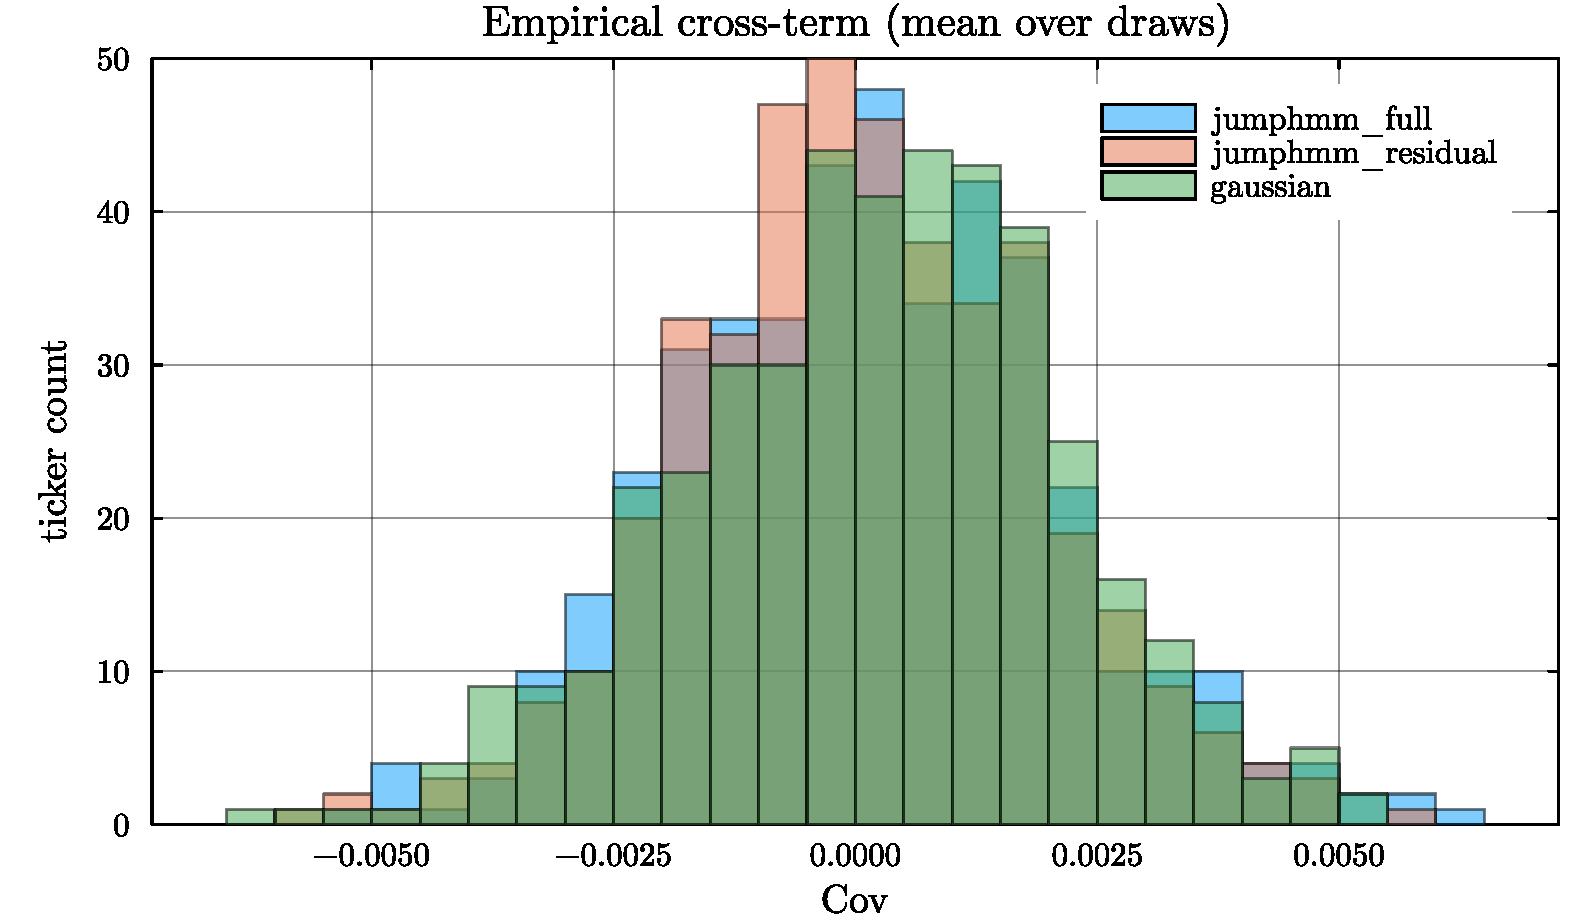
\includegraphics[width=0.85\textwidth]{figs/figS1_cov_diagnostic.pdf}
  \caption{\textbf{Empirical normalized cross-covariance
    $\Cov[\teps_i, g_m] / (\sigma_{\teps,i}\, \sigma_m)$ across
    the $423$-ticker universe.} Histograms were stacked per generator,
    with each per-ticker value averaged over $R = 100$ innovation
    draws. The full-return JumpHMM, residual-fit JumpHMM, and
    Gaussian generators all clustered at zero, validating the
    independence assumption used to derive Eq.~\eqref{eq:scale}.}
  \label{fig:cov_diag}
\end{figure}

% =============================================================================
% S2  Bias correction for daily-rebalanced backtests
% Four flat paragraphs:
%   (1) origin of the artifact (Booth-Fama identity + iid residuals)
%   (2) empirical demonstration on a 20-asset allocator
%   (3) the location-shift correction (formula, anchor, smoke test)
%   (4) rejected alternatives + downstream-use guidance
% =============================================================================

\section{Bias correction for daily-rebalanced backtests}
\label{sec:supp-bias}

The synthetic paths described in the main text reproduce per-asset
marginals and single-factor cross-sectional dependence faithfully but
discard temporal structure in the residual draw: at each trading day
the per-asset residual $\eps_i(t)$ is sampled independently from the
previous day. Real equity residuals carry a small but positive serial
autocorrelation \cite{loMacKinlay1990}, typically $\rho \in
[0.05, 0.10]$ at the daily horizon, so the iid-residual generator
family used here drops a real feature of the data. That omission
would be inconsequential for downstream tasks whose targets are
static (marginal fidelity, factor recovery, single-period
Value-at-Risk), but it creates a quantitatively large artifact for
backtests that rebalance at high frequency. A daily-rebalanced
portfolio with fixed target weights $w_i$ over $N$ assets has an
expected log-growth rate that, to second order, decomposes as
\begin{equation}
\E\!\left[\log \frac{W(t+1)}{W(t)}\right]
  \;\approx\;
  \sum_{i=1}^{N} w_i\,\mu_i
  \;-\; \tfrac{1}{2}\,\sigma_p^2
  \;+\; \tfrac{1}{2}\sum_{i=1}^{N} w_i\,\sigma_i^2,
\label{eq:booth-fama}
\end{equation}
where $\mu_i$ and $\sigma_i^2$ are the per-asset growth-rate mean and
variance and $\sigma_p^2 = w^\top \Sigma w$ is the portfolio
variance \cite{boothFama1992, markowitz1976longRun}. The non-negative
term $\tfrac{1}{2}\big(\sum_i w_i \sigma_i^2 - \sigma_p^2\big)$ is
the \emph{diversification return}: a structural bonus the
daily-rebalancing rule extracts mechanically by selling assets whose
weight has drifted above target (which on average have just risen)
and buying those whose weight has drifted below target (which on
average have just fallen). In real markets this buy-low/sell-high
mechanism trades into the positive residual autocorrelation noted
above, which partly offsets the bonus and shrinks the empirical
diversification return to a single-digit percentage point per year
depending on rebalancing horizon and cross-section
\cite{boucheyGunthorpSutherland2012}. Under independent draws the
autocorrelation is exactly zero and the rebalancing rule collects
the full structural premium of Eq.~\eqref{eq:booth-fama} unhedged,
inflating the median compound growth rate of any deployed allocator
on synthetic paths.

To anchor the scale of the artifact, we deployed a $20$-asset
long-only target-weight allocator (calibration window
$2014$--$2024$, deployment year $2025$, names with calibrated
$(\alpha, \beta)$ and $\max\beta = 1.21$, $5$~basis-point
round-trip cost) against the hybrid-composed universe of the main
text and decomposed the realized continuously compounded growth
rate (CCGR) into static and rebalancing-driven components.
Equal-weight buy-and-hold across the $20$ names produced
$\sim\!7.7\%/\mathrm{yr}$, a passive baseline for context. The same
target-weight allocation held statically for the deployment year,
with no intra-year rebalance, produced $\sim\!2.0\%/\mathrm{yr}$,
reflecting the marginal contribution of the chosen weights net of
costs. Switching the same allocation rule to daily rebalancing,
with no signal beyond the target weights themselves, produced
$\sim\!29.7\%/\mathrm{yr}$, a $+27.7$ percentage-point jump that
isolates the diversification-return term of
Eq.~\eqref{eq:booth-fama}. Adding a signal on top of the daily
rebalance moved the headline by a further $+0.13$~pp, immaterial
compared with the rebalancing-driven bonus. Deploying the same
allocator on the real $2025$ growth-rate history produced
$11.5\%/\mathrm{yr}$, so the synthetic median CCGR ran
$\sim\!22$~percentage points above reality. The decomposition makes
clear that the gap is a structural feature of the iid-residual
generator family rather than a calibration error: the allocator
choice, the cost model, the marginal calibration, and the
cross-sectional structure all behave on synthetic paths exactly as
they behave on real data; only the temporal structure of the
residual draw differs.

Because the artifact acts as a uniform multiplicative drag on the
path in log-wealth space rather than a distortion of the path's
shape, a uniform location-shift correction in the same space
restores the median absolute level without disturbing the rank
order, the drawdown geometry, or the volatility envelope of the
synthetic ensemble. Multiplying each path-$p$ wealth trajectory
$W_{p,t}$ at integer step $t$ by a uniform exponential drag whose
rate $b$ closes the gap between the engine's median annualized
growth rate and an external long-run prior
$\mathrm{CCGR}^{\mathrm{prior}}$,
\begin{equation}
\label{eq:bias-correction}
  W_{p,t}^{\mathrm{corr}} \;=\; W_{p,t}\cdot
  \exp\!\Big(\!-\tfrac{b}{100}\,\cdot t\,\Delta t\Big),
  \qquad
  b \;=\; \operatorname*{median}_{p}\mathrm{CCGR}_p \;-\; \mathrm{CCGR}^{\mathrm{prior}},
\end{equation}
with $\Delta t$ the integration step in years, accomplishes exactly
this. Working in $\log$-space rather than additively keeps the
correction multiplicative on wealth, which is the natural scale
for compounding returns and preserves drawdown geometry
period-by-period; the transform is monotone in $W_{p,t}$ for every
path and every step, so per-path rank order on terminal wealth is
preserved exactly. The prior $\mathrm{CCGR}^{\mathrm{prior}}$ is
set from external long-run data and is typically near
$8\%/\mathrm{yr}$ at the time of writing, decomposable into the
prevailing risk-free rate (roughly $4.5\%/\mathrm{yr}$ on a
five-year Treasury basis), the historical long-run equity premium
of $4$--$6$~pp \cite{damodaranERP, ibbotsonSBBI}, less $1$--$2$~pp
for fees, turnover, and market-impact frictions, leaving
$\sim\!3.5$~pp of active premium net of costs. Anchoring to a
documented prior rather than to the realized test-year outcome
avoids circular calibration: anchoring to the realized year would
force the synthetic median to collapse onto the test sample by
construction and would misrepresent typical years (in our
deployment, the realized $2025$ was an above-typical equity year,
so anchoring to its $11.5\%/\mathrm{yr}$ outcome would have
suppressed the corrected ensemble below its appropriate long-run
level). On a $200$-path smoke test the engine-raw median was
$29.78\%/\mathrm{yr}$, the bias drag was $b = 21.78$ percentage
points, the corrected median matched the prior at
$8.00\%/\mathrm{yr}$, and the real-$2025$ outcome landed at the
$63$rd percentile of the corrected ensemble, consistent with an
above-typical year (P5 $\approx -9\%$ for a bad year,
P50 $= 8\%$ for a typical year, P95 $\approx +25\%$ for a great
year).

Several alternative fixes were considered and rejected. A
path-filtering rule that drops synthetic paths above a CCGR
threshold turns the threshold itself into a target the audience
will probe and does not remove the structural artifact, merely a
subset of its consequences. Inflating per-trade transaction costs
to absorb the bonus would require round-trip costs of
$\sim\!70$~basis points versus the realistic $1$--$10$~basis points
seen on liquid US equity, and transfers a misrepresentation from
``the engine is great'' to ``costs are huge''. Drifting the
calibrated parameters between calibration and deployment to widen
the predictive envelope, with drift scale varied across
$\{0, 1, 2, 3, 5\}$ multiples of the OLS standard error, moved the
median Sharpe ratio from $2.02$ to $2.03$ across the sweep,
confirming that $\beta$ is estimated too tightly for SE-scale
drift to absorb the artifact. Imposing an AR(1) on the residual
draw inside the existing pipeline would conflict with the copula
reorder step, which destroys temporal structure by construction;
recovering the AR(1) requires a block-ordered copula sampler,
which is a structural redesign rather than a downstream
correction. The block bootstrap of empirical
residuals~\cite{politisRomano1994} preserves both temporal and
cross-sectional structure of the residual series by construction
and is a valid alternative generator pipeline, listed as a
future-work item that replaces the JumpHMM marginal rather than
correcting it. A multiplicative haircut on the engine-versus-static
deviation,
$W^{\mathrm{corr}} = W_{\mathrm{static}}\cdot
   (W_{\mathrm{engine}}/W_{\mathrm{static}})^{k}$, hits the same
anchor at $k$ chosen to match the prior but the rank correlation
with the raw engine drops to $0.748$ (paths reorder under the
correction) and the corrected drawdown distribution inherits
static-allocation geometry (median drawdown jumps from $5\%$ to
$9\%$, P95 from $13.5\%$ to $19\%$); we do not recommend it. The
corrected ensemble remains reliable for the ensemble-shape
analyses the paper validates: percentile diagnostics overlaying
real outcomes against the synthetic distribution, drawdown
distribution and tail-shape analysis, and relative ranking of
strategies evaluated on the same corrected paths. It does not
remove the underlying iid-residual limitation, so it does not
support workflows where residual autocorrelation is itself the
quantity of interest, where forward-prediction claims on absolute
Sharpe at daily rebalancing frequency are load-bearing, or where
the optimal rebalancing frequency is the question being asked;
for those workflows the AR(1) or GARCH residual structure
restructured around the copula reorder, listed as future work in
the Conclusion, is the appropriate path.

% =============================================================================
% S3 Validation metric definitions (KS, AD, W1, Hellinger)
% =============================================================================

\section{Validation metric definitions}
\label{sec:supp-validation}

The distributional and tail metrics reported in the main results
were defined as follows. The two-sample Kolmogorov-Smirnov statistic
between the empirical CDFs of the observed and simulated growth-rate
samples ($G_{\rm obs}$ of length $n$ and $G_{\rm sim}$ of length $m$)
is $D = \sup_x |F_n(x) - F_m(x)|$ \cite{kolmogorov1933, smirnov1948};
the test rejects when $D$ exceeds the critical value at level
$\alpha = 0.05$. The Anderson-Darling statistic places greater weight
on the tails via the integral
$A^2 = nm/(n+m) \int [F_n(x) - F_m(x)]^2 / [F(x)(1-F(x))] \, dF(x)$,
where $F$ is the pooled empirical CDF \cite{andersonDarling1952}. The
Wasserstein-$1$ distance between two empirical distributions of equal
length is the average of sorted-quantile differences:
\begin{equation}
W_1 = \frac{1}{n} \sum_{i=1}^{n} \big| G_{\rm obs}^{(i)} - G_{\rm sim}^{(i)} \big|,
\label{eq:wasserstein}
\end{equation}
with $G^{(i)}$ the $i$th order statistic. The Hill upper-tail index is the classical
order-statistic estimator
\begin{equation}
\hat\xi = \frac{1}{k-1} \sum_{i=1}^{k-1}
  \log\!\left( \frac{X_{(i)}}{X_{(k)}} \right),
\label{eq:hill}
\end{equation}
with $X_{(1)} \ge X_{(2)} \ge \dots$ the ordered upper-tail
absolute returns; $k$ is set to the upper $5\%$ of the
sample. For a Pareto-tailed distribution with shape $\alpha$,
$\hat\xi \approx 1/\alpha$. The Hellinger distance between two
density estimates $p$ and $q$ on a common bin grid is
\begin{equation}
H(p, q) = \frac{1}{\sqrt{2}} \, \Big\| \sqrt{p} - \sqrt{q} \Big\|_2
\;\in\; [0, 1],
\label{eq:hellinger}
\end{equation}
with $H = 0$ for identical densities and $H = 1$ for disjoint supports.

% =============================================================================
% S4 HMM-WJ simulator and grid-search pseudocode
% =============================================================================

\section{HMM-WJ simulator and grid-search pseudocode}
\label{sec:supp-pseudo}

The hybrid hidden Markov simulator described in the main text proceeded
as follows. Given fitted parameters
$(\mathbf{T}, \mathbf{E}, \bar{\pi}, \epsilon, \lambda, p_{\rm neg},
N_{\rm tail})$ and a horizon $T$:
\begin{enumerate}
  \item Draw $X_0 \sim \bar{\pi}$.
  \item For $n = 1, \ldots, T$: with probability $1 - \epsilon$, draw
        $X_n \sim \mathbf{T}_{X_{n-1}, \cdot}$; with probability
        $\epsilon$, sample $K \sim \mathrm{Poisson}(\lambda)$, and for
        the next $\min(K, T - n)$ steps force
        $X_n \sim \mathrm{Uniform}(\mathcal{S}_{-})$ with probability
        $p_{\rm neg}$ or
        $X_n \sim \mathrm{Uniform}(\mathcal{S}_{+})$ with probability
        $1 - p_{\rm neg}$.
  \item For each $X_n$, sample
        $O_n \sim \mu_{X_n} + \sigma_{X_n} \cdot t_5$.
\end{enumerate}
The grid-search procedure for $(\epsilon, \lambda)$ minimized
Eq.~\eqref{eq:grid_search} via brute-force evaluation over
$\{\epsilon_1, \ldots, \epsilon_K\} \times \{\lambda_1, \ldots, \lambda_L\}$,
with $200$ independent simulated paths per grid point and the
objective averaged over the path ensemble. The implementation lives in
the released \texttt{JumpHMM.jl} library at
\url{https://github.com/varnerlab/JumpHMM.jl}.

% =============================================================================
% S5 Transition matrix internals
% =============================================================================

\section{Transition matrix internals and partition diagnostics}
\label{sec:supp-transitions}

The fitted SPY transition matrix exhibited a dominant near-diagonal
band reflecting short-range regime persistence: row-sum entropy peaked
at the central states, and most off-diagonal mass was concentrated
within $\pm 5$ states of the diagonal. Tail-state exit probabilities
were systematically lower than central-state exit probabilities by
roughly an order of magnitude, which is what caused the volatility
clustering loss flagged by Bulla and Bulla \cite{bullaBulla2006} and
which the Poisson jump override addressed by re-injecting tail-state
mass independently of the empirical transition kernel. Quantile-bin
occupancy was approximately uniform over the in-sample window
($N = 100$), consistent with the Laplace fit's calibration to the
empirical CDF; the residual sample-size variation across bins was
smaller than the within-bin emission variance, so all $100$ states
received adequate statistical support. The full transition matrix and
partition-occupancy histograms are available in the released
\texttt{JumpHMM.jl/paper/} subdirectory.

% =============================================================================
% S6 State-resolution sensitivity
% =============================================================================

\section{State-resolution sensitivity}
\label{sec:supp-sensitivity}

We swept the partition resolution over
$N \in \{30, 60, 90, 100, 150, 200, 350\}$ and re-evaluated the
in-sample KS and AD pass rates for HMM-NJ and HMM-WJ. Pass rates were
flat across $N \in \{60, \ldots, 200\}$ with sub-percent variation,
indicating that the model was insensitive to partition resolution in
this range. At $N = 30$ both models lost approximately $5$ percentage
points on the AD test, reflecting the coarser quantile bins'
reduced ability to track tail behavior. At $N = 350$ several quantile
bins were never visited in the historical record, leaving the
corresponding emission parameters undefined; this set the practical
upper bound on $N$ for the SPY in-sample window. We adopted $N = 100$
as the operating point for all subsequent experiments.

% =============================================================================
% S7 Cross-asset generalization (NVDA, JNJ, JPM)
% =============================================================================

\section{Cross-asset generalization}
\label{sec:supp-cross-asset}

To verify that the hybrid HMM framework generalized beyond SPY, we
re-ran the full fit-and-validate pipeline on three single-stock
tickers chosen to span sector and volatility regimes: NVDA
(semiconductors, high volatility), JNJ (consumer staples, low
volatility), and JPM (financials, moderate volatility). Per-ticker
grid-search optimal $(\epsilon^{*}, \lambda^{*})$ adapted to each
asset's empirical clustering intensity, with $\lambda^{*}$ ranging
from $80$ (NVDA) to $130$ (JNJ); the $\epsilon^{*}$ stayed at the
lower boundary $10^{-4}$ for all three, consistent with the SPY
result. In-sample KS pass rates for HMM-WJ were $96.0\%$ (NVDA),
$98.2\%$ (JNJ), and $97.4\%$ (JPM), and out-of-sample pass rates were
$92.8\%$, $94.1\%$, and $93.5\%$, respectively. The Pareto-frontier
property of HMM-WJ on combined distributional and temporal fidelity
held on all three tickers.
